%--------------------------------------------------------------------------------------------------
%------------------------------------------------- Chapter --------------------------------------------------------

\chapter{Dispositivo Hipermedial Dinámico: Marco General}\label{cap:dhd} \label{cap:2}
%\pagenumbering{arabic}

\section{Introducción}

Este capítulo presenta el marco conceptual del Dispositivo Hipermedial Dinámico
(DHD) construido bajo una metodología de trabajo interdisciplinario, que ha
posibilitado abordar la problemática del campo disciplinar de la presente Tesis
contextualizadamente. A continuación se expone la definición conceptual del DHD:

\begin{quote} \label{definiciondhd}

Un Dispositivo Hipermedial Dinámico -DHD- es una red
heterogénea conformada por la conjunción de tecnologías y aspectos sociales (red sociotécnica) que
posibilita a los sujetos realizar con el otro acciones en interacción
responsable para \textit{investigar}, \textit{aprender}, \textit{dialogar},
\textit{confrontar}, \textit{componer}, \textit{evaluar}, diseminar bajo la
modalidad de taller físico-virtual, utilizando la potencialidad comunicacional,
transformadora y abierta de las TIC, regulados según el caso, por una
“coordinación de contratos”.

\begin{flushright}
(Sán Martín, et. al., 2008)\end{flushright}
\end{quote} 

Seguidamente se plantearán aspectos claves que han configurado la noción de DHD, observándose luego los actuales límites computacionales para dar solución a la totalidad de los Requerimientos del DHD.

La perspectiva teórica y metodológica del DHD se ha propuesto a través del Programa de Investigación, Desarrollo y Transferencia
“Dispositivos Hipermediales Dinámicos” –\url{http://www.mesadearena.edu.ar}-
(CIFASIS: CONICET-UNR-UPCAM), que lleva adelante desde el 2008 tareas de I+D+T. Específicamente el proyecto acreditado "Obra Abierta: Dispositivos Hipermediales Dinámicos para educar e
investigar” (CONICET-UNR), es el que desarrolla e implementa el estudio de la red sociotécnica en el marco de las organizaciones. Los ejes de I+D del programa son:

\begin{itemize}
\item La modalidad de taller físico-virtual en diversos contextos
organizacionales.
\item El modo interactivo-intersubjetivo de la red sociotécnica.
\item La teoría de los “Sistemas Complejos” para el estudio de casos y modelado
del DHD.
\item La teoría de “Coordinación de contratos” para el modelado de una pieza de
software bajo la perspectiva context-aware dinámico.
\item Sistemas de agentes de software para actuar en ambientes dinámicos
inciertos.
\item Herramientas y aplicaciones Web colaborativas.
\item Diseño de interfaces y heurísticas.
\item Repositorios institucionales de Acceso Abierto para la publicación de
materiales de Ciencia, Tecnología y Educación. Gestión de la Información.
\item La formación especializada en la crítica y difusión de las artes a través
del DHD.
\item Participación ciudadana mediatizada por DHD
\end{itemize}


Algunos de estos ejes son transversales a los diferentes proyectos de investigación en curso del Programa y vinculan,
entre otros, los principales planos que componen al DHD. Estos planos han sido diseñados para esta tesis con el propósito de facilitar la comprensión de cómo se ha elaborado el marco teórico y metodológico general. Cada uno de los planos configura
elementos que permiten el análisis diferenciado desde los distintos marcos disciplinares pero que a su vez habilitan el diálogo y la construcción de lo interdisciplinar. 

\subsection{El plano de las interacciones del DHD} \label{interacciones}

El plano 1 es abordado en la tesis doctoral "\textit{El Modo Interactivo Del
Dispositivo Hipermedial Dinámico}" cuya autora es la psicóloga Griselda Guarnieri,
(Dir. Dra. Patricia San Martín, Codir. Dr. Oscar Traversa). De esta tesis
se exponen a continuación los conceptos más relevantes sobre lo que se plantea
como interactividad responsable en el DHD.

Según Guarnieri (2010), el problema de investigación que aborda su tesis se centra en el estudio de las
interacciones que se suscitan en la trama compleja que se configura cuando los
sujetos se encuentran mediados/mediatizados en su comunicación y producción por
las actuales posibilidades de las Tecnologías de la Información y Comunicación
(TIC´s). 

Esto implica el estudio de las \textbf{interacciones} a través de sus definiciones,
\textit{caracterización}, \textit{contextualización}, \textit{medición} y
\textit{análisis}. Cada uno de estos elementos establece las referencias de
contacto con otros hiperplanos y proveerán parte de las restricciones y
requisitos que conforman los Requerimientos DHD.

\subsubsection{Las interacciones} \label{relaciones}

De las múltiples concepciones sobre interactividad en relación a la utilización de TIC se señalarán sólo algunas que resultan significativas a las argumentaciones para una mejor comprensión de la construcción conceptual.
La más elemental concibe la interactividad en el análisis de la relación entre el individuo y la computadora. Esta
concepción era plausible antes del advenimiento de internet,
un ejemplo de la cotidianeidad eran las situaciones lúdicas que experimentaban los usuarios en soledad con la
computadora en la pasada década. Actualmente es extraño que alguien lo haga de esta forma,
generalmente, las actividades de esparcimiento se realizan en red. Más allá de
entrenamientos o capacitaciones específicas con sistemas expertos y de
simulación con alto grado de automatizaciones que también hoy pueden estar en
red, cuando se plantea la interacción bajo perspectivas constructivistas del
conocimiento, se asume un sujeto dialógico constructor de contenidos, que
despliega sus capacidades críticas en el propio acto responsable, acto social instituido en la presencia de un otro.
Desde esta perspectiva, existen autores que han tenido en cuenta opciones más amplias para
definir la interactividad y consideran que esta no se agota a la relación
individuo-computadora, sino que implica también al vínculo mediado entre los
sujetos. 

\begin{defi} [ContratoDHD]

Un ContratoDHD es un dise\~no de contrato seg´un Meyer, bajos la filosof´ia de
"Design by Contract"


Retomaremos una definición de interactividad como la capacidad gradual y
variable que tiene un medio de comunicación para darle a los sujetos
un mayor poder tanto en la selección de contenidos (interactividad selectiva)
como en las posibilidades de expresión y comunicación (interactividad
comunicativa) \cite{lxxiv}.
\end{defi} 

En este sentido, la interactividad selectiva está vinculada principalmente a las posibilidades de
selección de contenidos. A diferencia de la interactividad selectiva, la
comunicativa se basa en que el usuario participe de intercambios dialógicos. “En
la interactividad selectiva, hay un individuo que pregunta o elige una opción y
el sistema le responde automáticamente; en la interactividad comunicativa, hay
un individuo emisor y otro receptor que pueden intercambiar roles. En el primer
caso, el número de posibilidades que tiene el sistema de responder es -por lo
menos en la mayoría de los casos limitado o a veces de una única manera;
mientras que en la segunda opción, la interacción es imprevisible, es decir las
posibilidades de respuesta son infinitas por las características humanas de los
interactuantes” \cite{lxxiv}.

Entonces, la interactividad comunicativa es mucho más difícil de cuantificar y medir que la interactividad
selectiva. Sin embargo, una noción actual de interactividad debe integrar y considerar ambas problemáticas, lo cual le otorga la dimensión de un vínculo intersubjetivo mediatizado por todas las posibilidades integradas que ofrecen las TIC.
En el caso de una interactividad contextualizada en procesos de educación, investigación y/o producción el vínculo intersubjetivo implica asumir dicha interactividad como acto responsable de parte de los sujetos participantes. No es sólo lo que se comunica, sino también lo que se produce tanto en forma individual como colectiva.

Es relevante observar que la interacción entre sujetos no se
puede separar de la comunicación, de la reciprocidad, "del compartir". La propuesta DHD
considera que ambos términos están interrelacionados, y que la interactividad
integra cuestiones propias del actual contexto físico-virtual visto como red
socio-técnica responsable.

En las últimas décadas, el término interactividad se ha entramado profundamente con la
digitalización, tanto de información, como de contenidos, por lo tanto no se puede pensar hoy
la interactividad separada de las posibilidades de intercambiar, modificar y
transmitir paquetes de información on line. A esto el posicionamiento del DHD
adhiere a las iniciativas mundiales de Acceso Abierto y Código Abierto a la
información y conocimiento como construcción de lo público plural y democrática.

La interactividad, a su vez, se fue distanciando de los dispositivos
transmisivos (unidireccionales), generando intercambios bidireccionales o
multidireccionales. Son innegables las posibilidades que ofrecen las TIC, pero cabe aclarar que
es necesario un profundo proceso de capacitación y resignificación de las
especificidades de su implementación y esa tarea es aún más compleja dado que
implica el cambio gradual de prácticas culturales que siempre son más lentas y
trabajosas que la velocidad de cambio y versatilidad de desarrollo de las TIC
(San Martín et al, 2010).

Siguiendo a San Matín (2003), las construcciones hipermediales y sus modos de organización son muy
diversos según la epistemología del dominio en el que se inscriban. Pero su
especificidad estructural está en la ausencia de un orden jerárquico que fije
previamente el dominio de su lectura y en la invención de nuevas formas.

Es necesario indagar, en el caso de las tecnologías informáticas, que
poseen todos los elementos para posibilitar un intercambio interactivo, si este
realmente se realiza. Durante el trayecto de investigación de la tesis mencionada
circunscrita al estudio del plano 1, se efectuaron análisis de diversas
implementaciones en el campo educativo mediatizado en distintos grados a través de internet y se ha
observado frecuentemente que se reemplaza el texto impreso en papel por
el digital, la fotocopiadora por el texto online, pero no hay verdaderos canales
que posibiliten la interactividad entre los usuarios.


\begin{defi} [Interactividad DHD] En resumen, conceptualizamos la Interactividad DHD
como un vínculo intersubjetivo responsable mediatizado por una las TIC que conforma una red sociotécnica que posibilita el
intercambio y edición bidireccional o multidireccional de mensajes y objetos en un marco de trabajo
colaborativo, abierto, democrático y plural.
\end{defi} \label{interactividadDHD}


\begin{figure}
\begin{center}
 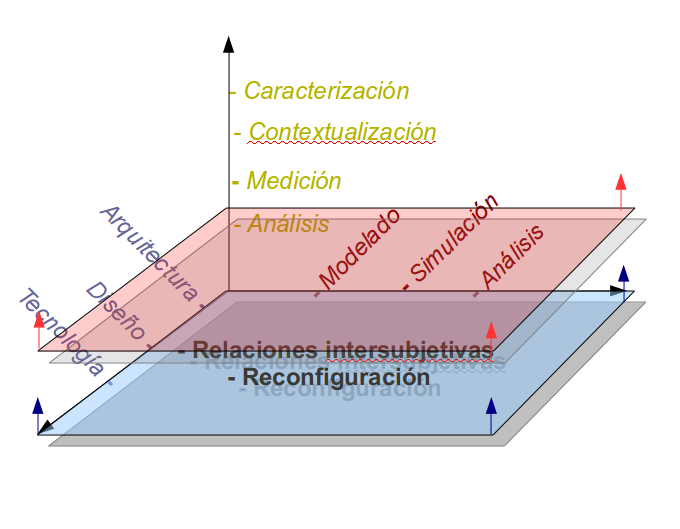
\includegraphics[width=4 in,totalheight=3 in] {DHD/hiperplanosDHD}
 % .: 0x0 pixel, 0dpi, 0.00x0.00 cm, bb=
\caption{Hiperplanos del los RequerimientosDHD} \label{hiperplanos}
\end{center}
\end{figure}


\subsection{El plano sistémico del DHD}

El plano 2 es abordado en la tesis doctoral "\textit{La Teoría De Los Sistemas
Complejos Aplicada Al Modelado Del Dispositivo Hipermedial Dinámico}" cuyo autor es el Ing. Guillermo Rodriguez (Dir. Dra. P. San Martín, Codir. Dr. J.C. Gomez). Esta tesis aportó la selección de una teoría de
modelado que contempla la necesidad de evaluación de las interacciones como
eventos diferentes en una base de tiempo continuo. La selección del formalismo
DEVS (Discrete EVent dynamics System) es presentada como una teoría específica que
conjuga ambas necesidades. A su vez, se aporta el desarrollo de
métricas cuali-cuantitativas en función del análisis evaluativo. La confección de la métrica
fue realizada en forma interdisciplinaria y por ende se ve reflejada en varios de los proyectos de tesis en curso sobre el DHD. Entonces, del estudio sistémico del DHD se desprende que a través del
\textit{modelado}, la \textit{simulación} y el \textit{análisis} es  posible
describir aspectos importantes de su conceptualización en virtud de sus
dinamismo sistémico.


\subsubsection{Dinamismo sistémico del DHD}

Se ha planteado el concepto de interactividad directamente vinculado a las
actuales posibilidades de 
vinculo social y herramientas tecnológicas que brindan las TIC.
Las formas de trabajo colaborativo plural y democrático, la edición sincrónica y
asincrónica, las varias herramientas de gestión y comunicación, la computación
distribuida brindan un escenario potencialmente apto para el desarrollo de
nuevas modalidades educativas, de gestión, investigación y producción.


Específicamente los sistemas hipermediales adaptativos tienen como
objetivo construir un espacio capaz de ajustarse a las particularidades de cada
actor, lo que constituye una forma única de interacción y reciprocidad
entre el sujeto y el sistema. Su naturaleza permite configurar entornos para lograr que
los participantes alcancen los objetivos establecidos mediante contenidos y
recorridos adecuados a sus aptitudes, intereses y preferencias.
Por lo tanto, estos sistemas buscan que el contexto se adapte al usuario y
no al contrario, como sucede en los hipermediales “clásicos”, los cuales
muestran el mismo contenido y los mismos enlaces a todos los usuarios. En
este sentido, para que el sistema sea adaptativo debe ser configurado en un entorno
hipermedial donde el usuario sea capaz de realizar dicha
adaptación \cite{lxxviii}.
 
Existe diferencia entre estos sistemas hipermediales adaptativos y un
sistema adaptable ya que éste último se enfoca, básicamente, en proporcionar
al usuario herramientas para la personalización del sistema (color, tipo de
letra, tamaño de letra, etc.), o en contar con interfaces para diferentes
niveles (por ejemplo, experto, principiante, etc.). De este modo, la gran
diferencia es que en un sistema adaptable, el usuario diseña su entorno
seleccionando según sus necesidades o intereses, mientras que un sistema
hipermedial adaptativo emplea un modelo de usuario para proveer adaptación
automática, aunque también estos últimos pueden contar con características
adaptables \cite{lxxviii}.

De modo general, se define a los sistemas hipermediales adaptativos
como sistemas hipermediales que permiten personalizarse (adaptarse) en
función de los usuario individuales. De este modo, el modelo se desarrolla a
partir de las metas, preferencias, características personales y conocimientos de
cada usuario, el cual lo utilizará y modificará según vaya interactuando con el
sistema y así adecuando la información (contenidos) y los links para la
navegación, a sus necesidades, ya que considera que los usuarios aumentan y
varían sus conocimientos permanentemente. Todo sistema a su vez, refiere a un
contexto, por lo que cabe aclarar que por “contexto” se entiende según Dey
a ``cualquier información que puede usarse para caracterizar la situación de
una entidad. Entendiendo a la entidad como una persona, lugar u objeto
que es considerado relevante para la interacción entre un usuario y una
aplicación, incluyendo al usuario mismo y la aplicación`` \cite{lxxix}.

De este modo, el contexto es información, y según como se selecciona, procesa y
produce la misma a través de dichos sistemas, se posibilita la adecuación del
mismo con las utilidades para el usuario. Dourish \cite{contexto} sostiene al
respecto que según la variable situación contextual en la cual la tecnología es
utilizada, se necesita comprender más sobre la relación entre la tecnología
informática y el contexto en la que se encuentra.

El problema del contexto no refiere a cómo se representa sino que tiene
que ver con un problema de relaciones, es decir, con qué se vincula la
actividad que se desarrolla, de las características del contexto en que se
desenvuelve y a su vez, cómo y porqué las personas que interactúan pueden
tener una comprensión mutua del contexto para sus acciones. La idea de
contexto consiste en un conjunto de características del mismo que rodean las
actividades que se realizan, y que estas características pueden ser codificadas
y hacer viable, de este modo, un sistema de software. Entonces, el contexto es lo que las personas
hacen y no la sola descripción de un escenario. Es un producto de la relación,
mas que una premisa. Así el contexto y la
actividad no pueden separarse. El contexto no es algo estable, dado, como una
descripción externa a la actividad misma. Por el contrario, aparece y es
sostenido por la misma actividad.

En síntesis, en el marco de este trabajo, el DHD debería ser sensible o adaptable al contexto para posibilitar el
dinamismo propio de las interacciones dadas en las comunidades de práctica.


\subsection{El plano de la Ingeniería Computacional del DHD} \label{plano3}

El plano 3 (figura \ref{hiperplanos}) conforma la base tecnológica y
computacional del DHD, establecida por la arquitectura, el diseño y la
tecnología utilizada para el desarrollo. Estos tres elementos involucran las
resoluciones funcionales de los requerimientos DHD. 


De esta manera se establece que en el marco tecnológico y disciplinar de los
siguientes capítulos que componen la presente tesis, cuando se refiere
al Dispositivo Hipermedial Dinámico se limita el alcance solamente a los
requerimientos funcionales, computacionales y de diseño, dando cuenta de la
imposibilidad de brindar soluciones a la totalidad de los elementos que devienen
de la construcción interdisciplinaria (\ref{definiciondhd}).


\subsubsection{Campo teórico-metodológico interdisciplinario del DHD}

Las tareas de investigación llevadas adelante desde el 2003 por el grupo de
investigación Obra Abierta en sus diferentes estudios de caso, refieren al
estudio de problemáticas vinculadas a la integración efectiva de las TIC, en
diferentes contextos organizacionales educativos tanto públicos
como empresariales (San Martín et al, 2008) fundamentándose en conceptos, método
y bases epistemológicas de la investigación interdisciplinaria en el marco de
los sistemas complejos (García, 2007).

Estos fundamentos posibilitaron, en la continuidad de los distintos proyectos,
la construcción de la noción de Dispositivo Hipermedial Dinámico (DHD) y la
conformación del programa ya mencionado que tiene por objetivo general
consolidar el marco teórico, metodológico y de desarrollo tecnológico
del DHD. En este sentido, el abordaje de las problemáticas se realiza como se
expuso en el parrafo anterior, implementando una metodología de investigación
interdisciplinaria que estudia el mismo como sistema complejo.

Siguiendo a San Martín y Guarnieri (2009), construir una red sociotécnica en un
contexto físico-virtual con “presencialidad” subjetiva es sentir la Presencia
del otro que cobra sentido en el compromiso de participación responsable para
enseñar y aprender, investigar y/o   producir  cualquiera    sea   el   grado   
y   tecnología de mediatización. Presencia que en su dimensión simbólica
posibilita el vínculo intersubjetivo y da lugar a la distancia necesaria para la
interrogación, la representación como “juego al pensamiento” (Enaudeau, 1999),
la mediación de los  discursos (Lasch, 2005) y la acción (Bruner, 2001). La
utilización o no de TIC en un determinado proceso educativo, investigativo
o de producción y el grado de mediación/mediatización de dicho proceso no puede 
ignorar el contexto del siglo XXI, que da muestra de los múltiples impactos de
la globalización. El problema relevante en una sociedad donde la interactividad
digital es un hecho consumado, es interrogar sobre cómo sostener la presencia
subjetiva y la participación ciudadana responsable e inclusiva. Estas  
dimensiones, pensadas como indisociables, podrían posibilitar quizás la
reflexión sobre la construcción de nuevos vínculos generadores de
“civitas” (Borja, 2006) más allá del grado de mediación/mediatización. Entonces,
la problemática así planteada excede el tradicional dualismo
presencial - a distancia y lo meramente cuantitativo del grado de mediatización,
centrándose el debate en su real dimensión política dada la emergencia de nuevas
formas culturales físico-virtuales de gestión, transmisión, producción y acceso
-o no- a la información y conocimiento. Esto involucra de hecho las
posibilidades de desarrollo tecnológico colaborativo y la extensiva utilización
abierta de herramientas digitales aptas para múltiples propósitos.


Partiendo de estos posicionamientos, se elaboraron aspectos referidos   a   
las condiciones    necesarias   para   el  que hacer interdisciplinario  en  el 
propio   campo    de   acción,  atendiendo a los fundamentos que sostienen la
construcción del marco conceptual común y a reflexiones acerca del desarrollo de
una práctica convergente que supone asumir una cierta distancia hacia los
problemas particulares de los propios    campos    disciplinares  para   lograr 
visualizarlos  desde  otras perspectivas menos conocidas situadas en el contexto
sistémico que se expresan. Este quehacer interdisciplinario demanda un necesario
corrimiento generador de  tensiones   tanto  a  nivel   subjetivo como
intersubjetivo entre la propia formación profesional especializada y la tarea
interdisciplinaria que habita en un caso que muestra una realidad dinámica
y dificultosa que no se detiene, constituyéndose dichas tensiones durante
el desarrollo de la investigación en un aspecto revelador de la integración
dinámica del grupo de trabajo. Siguiendo a García (2007) se acuerda que la forma
en que se van generando esas necesarias tensiones puede condicionar
significativamente la calidad de los resultados
producidosinterdisciplinariamente. Surgen así interrogaciones sobre las
posibilidades y limitaciones de ese necesario corrimiento y se desarrolla la
construcción de una  metáfora del DHD: “la mesa de arena”. Esta metáfora ha sido
presentada por San Martín y Guarnieri (2009) como plano de pensamiento del arte,
proyectándose como interferencia intrínseca al plano filosófico del concepto de
dispositivo y al plano científico de los sistemas complejos y, como
interferencia extrínseca del pensamiento creativo tecnológico. En referencia
directa a esta tesis, esto significa que las cuestiones tecnológicas y
computacionales están fuertemente involucradas en los requierimientos de los
DHD, pero son insuficientes para el abordaje del plano filosófico sobre lo que
se entiende conceptualmente como dispositivo. 


La noción de dispositivo, como señala Traversa (2001), tiene un
campo de aplicación extenso y su empleo puede encontrarse en disciplinas
tales como la filosofía, la mecánica, la informática, la comunicación, la
sociología, la educación, el arte, etcétera, presentando perspectivas
analíticas diversas (Deleuze, 1990; Agamben, 2007; Meunier, 2007). Sus
alcances abarcan  desde mecanismos y  componentes tangibles a
configuraciones de un alto grado de abstracción. En este último sentido
Foucault lo conceptualiza como un conjunto heterogéneo:
      
      
\begin{quote} 
      “(...) lo que quisiera señalar en el dispositivo es justamente la
      naturaleza del vínculo que puede existir entre esos elementos
      heterogéneos. (...) entre dichos elementos –discursivos o no
      discursivos- existe algo así como un juego, cambios de posición,
      modificaciones de funciones, que pueden,también ellos, ser muy
      diferentes”. (Foucault: 1991, 185).
\end{quote} 

Siguiendo a Foucault, se adopta una visión que asume lo heterogéneo de los
elementos y sus modos de vinculación que entraman concepciones de
poder y sujeto del saber. El dispositivo se manifiesta entonces, como una
entidad compleja compuesta por la integración de dos dimensiones
indisociables: una técnica (o conjunto de técnicas constructivas que
comportan una materialidad y una configuración particular) y una social
dada por las relaciones intersubjetivas y la situación en la que se
inscriben. Este concepto da cuenta de la presencia dinámica de tecnologías, vínculos
interactivos/intersubjetivos y representaciones como lugar en que operan los
intercambios discursivos, potencial espacio para la co-enunciación ya
que se torna posible el emplazamiento social de los discursos.
\label{intersubjetivas}

Retomando la metáfora de "la mesa de arena" como lugar de interacción múltiple,
léase un plano sustentador físico-virtual que posibilita realizar
responsablemente ensamblajes de elementos heterogéneos a través de operaciones
complejas, donde es posible conversar y dialogar mientras se construye e integra
conocimiento con ideas creativas y diversos elementos, materiales o herramientas
disponibles; el DHD propone habitar un lugar de acción reflexiva, de enunciado
de hipótesis, de observación detenida, de participación activa para vivenciar
la virtualidad de las ideas y a la vez admitir el error para volver a comenzar.
Así, se hace imprescindible vincular la dimensión contextual de cada sujeto
participante en su más amplio sentido, como variable que condiciona los procesos
y calidad de las interacciones. Se trata entonces, de habilitar la evaluación
reflexiva y continua sobre lo que se aprende, se enseña, se investiga y se
produce: el valor y el sentido de lo que se comunica y disemina para construir
“civitas”. De allí, este enfoque difiere cualitativamente de la administración,
gestión y comunicación de la información, dado que si bien la incluye, atiende a
una dimensión ética que excede lo meramente informacional.

En la metodología de trabajo propuesta, los conceptos guían a los procesos y a
la interevaluación permanente de los mismos y de sus productos asociados como
dinámica propia del desarrollo de conocimiento y del compromiso hacia el otro.
Así, el despliegue de la red sociotécnica, trasciende lo meramente 
instrumental, posibilitando mediaciones y mediatizaciones sustentadas en un
conocimiento profundo de los propósitos que habilitan la construcción de un
campo de responsabilidad efecto de la interacción social participativa, en el
marco del constructivismo dialéctico (Vygotsky; 1988) y la modalidad pedagógica
de taller. En este sentido San Martín (2009), ha desplegado una visión no
instrumental y crítica considerando a las   “competencias  profesionales”  
requeridas, como capacidades que se sintetizan en el sujeto como el “saber hacer
– saber ser”, que más allá de la singularidad disciplinar se construyen e
integran en profundidad como un saber “ha-ser” ético, manifestado en una actitud
responsable hacia la calidad de la existencia asumiendo la diversidad y la
complejidad del contexto físico-virtual, expresándose en los planos científicos,
artísticos y técnicos a través de articuladas coordenadas de acción. La noción
de DHD para educar, investigar y producir en el contexto físico-virtual
conceptualiza a la educación  y/o   investigación  (cualquiera   sea   su    
grado de mediación/mediatización) como proceso   complejo que  involucra   la
constitución misma de los sujetos que la piensan, en su más profunda dimensión
ética.

Entonces, para favorecer la alternativa del saber “ha-ser” ético, se hizo necesario
construir una perspectiva  organizacional, pedagógica, investigativa y de
desarrollo tecnológico, poniendo en obra una metodología interdisciplinaria que
sustentara el estudio del sistema complejo para abordar los problemas desde
su contexto real situacional. Esta aproximación solicita teorías y técnicas
reflexivas de acción participativa por parte de todos los actores
involucrados para el tratamiento de los mismos en su complejidad. El supuesto
se basa en que dicha participación físico-virtual en el propio tratamiento
metodológico de las problemáticas sustentada en el marco epistemológico de los
sistemas complejos, habilitaría la necesidad de desarrollo de originales
síntesis de acción (multiplicidad metodológica-prácticas
convergentes) posibilitando tal vez la alternativa de enfrentarse y afrontar la
responsabilidad ética, asumir responsabilidad por esta responsabilidad.

Cabe aclarar que esta perspectiva sobre los sistemas complejos, confronta con
aquellas “soluciones” informáticas donde sistemas tutoriales inteligentes (STI),
determinan pasos claves en la metodología de una propuesta educativa,
investigativa y/u organizacional centrada en la linealidad
causa-efecto. Es evidente también que no se  adhiere  a  soluciones
donde   el  diseño “instruccional”, desarrollo de contenidos, materiales
didácticos (objetos digitales educativos) y administración de plataforma, están bajo
un modelo terciarizado quedando determinaciones y desarrollos claves a cargo
de personas ajenas a la institución/organización. En ambos casos, es observable
que no se capitalizan las posibilidades de desempeño profesional y crecimiento
de los responsables (la trama institucional conformada por todos sus actores,   
especialmente docentes, investigadores y profesionales), al reconocimiento de la
diversidad y necesario vínculo intersubjetivo singular con quienes se están
formando, evidenciándose a nivel institucional, la ausencia del diseño y
desarrollo de una política académica de formación  permanente, de
promoción del diálogo y reconocimiento de las propias capacidades de la
organización.

Dado todo lo expuesto, en la observción del plano 2 de la figura
\ref{hiperplanos} se visualiza que:
     
\begin{quote}
     “La complejidad de un sistema no está solamente determinada por la
     heterogeneidad de los elementos (subsistemas) que lo componen, y cuya
     naturaleza los sitúa normalmente dentro del dominio de diversas ramas de la
     ciencia y la tecnología. Además de la heterogeneidad, la característica
     determinante de un sistema complejo es la interdefinibilidad y mutua
     dependencia de las funciones que cumplen dichos elementos dentro del
     sistema total. Esta característica excluye la posibilidad de obtener
     un análisis de un sistema complejo por la simple adición de estudios
     sectoriales correspondientes a cada uno de los elementos.” 
     \begin{flushright} (García, 2007,87)     \end{flushright}
\end{quote} 

Por lo tanto, como exponen Rodriguez y San Martín (2010), la funcionalidad
global de un sistema se da precisamente por las interacciones y no se encontrará
tal funcionalidad si se observan solamente algunos elementos. Es debido a esto
que dicha funcionalidad se denomina “emergente”, dado que solo se encuentra
a nivel sistema (Bar-Yam, 1997). Además, el sistema como totalidad es abierto,
no tiene contornos rígidos; está inmerso en una realidad más amplia con la cual
interactúa por medio de flujos heterogéneos de categorías diversas.


El sistema complejo no es algo ya dado que no hay más que observar y analizar,
sino que demanda un esfuerzo en la investigación para su conceptualización como
recorte posible de una realidad mucho más amplia e indefinible en sus límites.
Esta construcción demanda una metodología que de lugar a la formalización de
modelos  sucesivos  donde   se  busca   una   aproximación  que   sea
suficientemente coherente en la capacidad de explicar el funcionamiento
de dicha construcción (sistema complejo) dando cuenta de los hechos
observados. Esta posibilidad de modelización del sistema complejo permite
comprender con mayor exactitud como el pensamiento científico conforma
un plano de referencia mediante proposiciones. Modelizaciones que se
definen a través de expresiones matemáticas, formalismos u órdenes
metodológicos híbridos cualitativos y cuantitativos donde el grado de
variabilidad  para definir la  complejidad  no  corresponde   a   lo
inconmesurable ya que lo complejo no es científicamente análogo a lo
caótico, aunque perceptualmente lo pareciera.



La multiplicidad de miradas analíticas y disciplinares que habilita el
DHD, permite observar que en el marco teórico de los sistemas complejos
refiere a un estado de cosas en un tiempo finito y en determinada realidad
contextual referenciable donde se puede accionar grupalmente para
efectuar cambios estructurales constatables, mientras que a su vez en un
plano absolutamente diferenciado, el DHD resuena como acontecimiento
en el pensamiento y subjetividad de los participantes. Así surge el desafío
de articular el intercambio con el otro (disciplinar) para descubrir, explorar
y construir grupalmente alternativas metodológicas que desde cada
singularidad desplieguen posibles “interferencias” intrínsecas o extrínsecas
para elaborar lo “significativamente común”.

Como dinámica de intercambio colaborativo, la modalidad de taller físico-vi
rtual permite un ámbito de aplicación donde el conocimiento se construye
participativamente tensionando con otros y con uno mismo en la propia
interrogación. Se plantea esta modalidad de trabajo como imprescindible para la
construcción de un contexto social y productivo físico-virtual inclusivo y
democrático propio de lo público. Atendiendo al plano de pensamiento de
desarrollo tecnológico, es posible desde lo disciplinar visualizar las
herramientas y sistemas informáticos que posibilitan trabajar colaborativamente
en el actual contexto físico-virtuale. Lo propuesto, intenta aportar un posible
camino hacia el análisis evaluativo sobre cómo se desarrollan y se podrían
mejorar procesos de interactividad responsable a través de redes sociotécnicas
para educar, investigar y producir. 


\section{Requerimientos DHD} \label{requerimientosdhd}

Esta sección se referencia en el marco de los procesos de la Teoría    
deRequerimientos (AGREGAR CITA) para abordar la problemática conceptual DHD que
presenta aspectos diferenciales a los usuales de requerimientos TIC. 

Se adopta una diferenciación sutil entre los términos "Requisitos" y "Requerimientos" que expresan dos
niveles relacionados cuando se abordan la resoluciones funcionales,
relacionales y reconfigurativas del DHD. Este planteo se realiza siguiendo a diferentes
proyectos \cite{requerimiento1,requerimiento2,requerimiento3,requerimiento4} que
utilizan en forma similar esta distinción.
En este sentido se incluyen ítems que tratan cuestiones
significativas: 

\begin{enumerate} \label{requerimientositems}
 \item  Determinación de Requisitos/requerimientos que total o parcialmente
no tienen solución computacional.
 
 \begin{enumerate}
 \item Aspectos de reconfiguración 
 \item Aspectos de interactividad responsable 
 \end{enumerate}
\item Determinación del propósito que impide la solución computacional.

\end{enumerate}

\begin{defi} [Requisito DHD]: 
Entonces, definimos como requisitos del DHD (RequisitosDHD) a
todas las características que implican tanto los aspectos sociales como tecnológicos del
DHD. Esto significa que si se representa una secuencia de "ejecución", por
ejemplo situada en un proceso educativo \cite{cacic2007}, a través de una
máquina de estado, la representación de cada uno de los estados deberían ser
descriptos a partir de los conceptos propios del DHD referidos a interactividad responsable, modalidad taller, dinamismo, reconfiguración,
coordinación, contextualización, etc.
\end{defi} \label{requisito}

Con la finalidad de ejemplificar Requisitos del DHD se plantea como escenario un curso de formación docente destinado a la elaboración de materiales educativos digitales, donde los destinatarios deben realizar reediciones colaborativas sobre Objetos Digitales Educativos (ODE) disponibles en Acceso Abierto.

\begin{ejemplo}
RequisitosDHD 1: El proceso físico-virtual de recontextualización y reedición colaborativa que realizan los alumnos sobre un ODE dado, debe quedar registrado para posibilitar la evaluación del grado de interactividad responsable de los alumnos involucrados. 
En el desarrollo de dicho proceso, si es necesario, el/la docente debe tener la posibilidad de cambiar dinámicamente estrategias didácticas, actividades relacionadas y la semántica de las interfases sin que estas últimas sufran modificaciones.
\end{ejemplo} \label{ejemplo1}

\begin{defi} [Requerimiento DHD]: Definimos como requerimientos del
DHD a la interpretaciones de los RequisitosDHD que puedan ser expresadas
mediantes modelos formados por componentes, tipos de componentes, relaciones
y tipos de relaciones que sirvan para especificar funcionalidades, conceptos,
patrones y estilos. Por cada RequisitoDHD puede haber varios RequerimientosDHD.
\end{defi}\label{requerimiento}
 
Como RequerimientosDHD derivados de los RequisitosDHD del ejemplo anterior se mencionan:

\begin{ejemplo}
RequerimientosDHD 1: El sistema debe proveer el mayor grado de información posible sobre las interacciones de la red sociotécnica, el porcentaje cuanti-cualitativo en el uso de los servicios de edición de las herramientas seleccionadas en el entorno virtual y el porcentaje de interacciones responsables que promovió cada usuario.
A su vez, se debe posibilitar que el usuario docente pueda cambiar en tiempo
de ejecución la funcionalidad de los servicios del foro a partir de información
de contexto del usuario alumno.
\end{ejemplo} \label{ejemplo2}


\subsection{Breves antecedentes sobre el tratamiento de requerimientos 2}

El tratamiento de requisitos/requerimientos es el proceso mediante el cual se especifican
y validan los servicios que debe proporcionar el sistema así como las
restricciones sobre las que se deberá operar. Consiste en un proceso iterativo
y cooperativo de análisis del problema, documentando los resultados en
una variedad de formatos y probando la exactitud del conocimiento
adquirido (Ferreira y Loucopoulos, 2001). La importancia de esta fase
esencial puesto que los errores más comunes y más costosos de reparar, así
como los que más tiempo consumen se deben a una inadecuada ingeniería de
requisitos.

Dados los límites de esta tesis, no se pretende desarrollar la problemática de la Teoría de
Requerimientos en general, sino sólo la breve descripción de algunos de los
procesos que se adecúan mejor a los requerimientosDHD. Este abordaje
permitirá exponer una caracterización indirecta de los requerimientosDHD,
proporcionando un aporte enriquecedor sobre otros requerimientos convencionales inherentes a la construcción de herramientas educativas basadas en tecnología Web. Según Lowe & Hall (1999), el proceso de especificación de requisitos se puede dividir en tres grandes actividades:

\begin{enumerate}
\item Captura de requisitos
\item Definición de requisitos
\item Validación de requisitos
\end{enumerate}


\begin{figure}
\begin{center}
 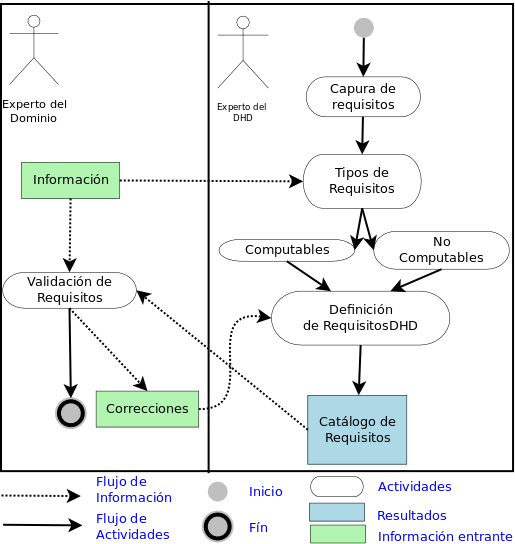
\includegraphics[width=4 in,totalheight=3 in] {DHD/ProcesoIngRequisitos}
 % .: 0x0 pixel, 0dpi, 0.00x0.00 cm, bb=
\caption{El proceso de Ingeniería de Requisitos} \label{fig:Requerimientos}
\end{center}
\end{figure}


\subsubsection{Captura de requisitos para los DHD}

La captura de requisitos es la actividad mediante la cual el equipo de desarrollo
de un sistema de software extrae, de cualquier fuente de información disponible,
las necesidades que debe cubrir dicho sistema (Díez, 2001). En los DHD el
proceso de captura de requisitos puede resultar complejo, principalmente por el marco conceptual complejo que sustenta la red sociotécnica para educar, investigar y/o producir.
Es observable la gestión de procesos dinámicos que requieren reconfiguraciones
propias de la modalidad participativa y colaborativa de taller. Esto supone
tanto a nivel tecnológico informático proporcionar un sistema flexible como a
nivel organizacional diseñar e implementar políticas de participación
responsable que implican altos niveles de abstracción no computables.
\label{no_computable}

A continuación se exponen sintéticamente dos técnicas para la captura de requisitos que resultan
pertinentes al DHD, a saber:

\begin{descrition}
\item [Casos de Uso:] Aunque inicialmente se desarrolló como técnica para la
definición de requisitos (Jacobson, 1995), algunos autores proponen casos de uso
como técnica para la captura de requisitos (Pan, Zhu & Johnson, 2001 y Liu &
Yu, 200). En ingeniería del software, un caso de uso  es una técnica para la
captura de requisitos potenciales de un nuevo sistema o una actualización de
software. Cada caso de uso proporciona uno o más escenarios que indican cómo
debería interactuar el sistema con el usuario o con otro sistema para conseguir
un objetivo específico. Normalmente, en los casos de usos se evita el empleo de
jergas técnicas, prefiriendo en su lugar un lenguaje más cercano al usuario
final. En ocasiones, se utiliza a usuarios sin experiencia junto a los
analistas para el desarrollo de casos de uso. Es en este sentido que la
metodología adoptada en varios de los proyectos que integran el Programa de
I+D+T "Dispositivos Hipermediales Dinámicos" considera centralmente el estudio
de caso contextualizado.


Siguiendo a Thomas et al (2008), en la perspectiva DHD se considera que los
procesos de producción y construcción social de la utilidad y el funcionamiento
de las tecnologías son indisociables y se configuran a partir de relevantes
intervenciones y estilos locales, tanto en el plano de la innovación tecnológica
como del desarrollo cognitivo ya que la utilidad de un artefacto o conocimiento
tecnológico está presente tanto en el diseño del artefacto como en los procesos
de re-significación de las tecnologías en los que participan diferentes grupos
sociales relevantes (investigadores, tecnólogos, usuarios, funcionarios
públicos, integrantes de ONG, etc.). 


\item [UWATc+:] Esta técnica fue especialmente creada para la toma de
requisitos de un DHD con finalidad educativa. Está orientada hacia la
creación de las reglas de coordinación de los contratos y a la
identificación del lugar donde debe conectarse el contrato teniendo en
cuenta el flujo de utilización de componentes dentro de un proceso educativo. En \cite{cacic2007} se presenta un primer diseño compresivo para el
modelado de los procesos de educación e-learning (Pe-lrn) en un Aplicación Web
E-learning con la inclusión de contratos con propiedades context-aware
\cite{libro}. El modelo está basado en UWAT+ (Distante, 2004), una versión
extendida y adaptada de ”UWA Transaction Design Model” para el diseño de
transacciones en aplicaciones Web. El principal aporte de UWATc+ es
el acercameinto de un modelo útil para la represetación de transacciones
e-learning en una AWe-lrn; permitiendo una mejor distinción de la ubicación
(entre servicio-usuario(s) y servicioservicio(s)) de la componente contrato
dentro del flujo de ejecución. Detalles de este desarrollo serán expuestos en el capítulo ....XXX
\end{description}


\subsection{Abstracción para el refinamiento de los RequerimientosDHD}

Por último es necesario hacer un refinamiento de los requerimientos
anteriormente mencionados para alcanzar una especificación funcional. De esta
manera, se pretende exponer cuáles son los elementos de primera clase que
integran las especificaciones y que son productos finales de refinamientos de
otros elementos que a su vez derivan de RequisitosDHD y RequerimientosDHD.

En la figura \ref{requerimientosdhd} se muestra una primera aproximación de
dichos elementos que intervienen en la etapa de refinamiento de los
requerimientos hacia la especificación funcional. Cada uno de los bloques
representan diferentes niveles de refinamiento, posibles de asociar a niveles de abstracción. El proceso de refinamiento de los
elementos se realiza sobre los componentes abstractos del \textit{Nivel 2}, 
a los cuales se les aplica unas primitivas de refinamiento para derivar los
respectivos modelos concretos. Dos tipos de refinamiento distinguen este
proceso:  

\begin{definition}
\item [\textbf{El refinamiento estructural}] se realiza sobre el modelo
abstracto de roles cualificado con unas relaciones de transformación que
permiten obtener el modelo concreto de roles. Se utilizan primitivas de
refinamiento como agregación, especialización, relación, que determinan el tipo
de transformación que se aplica sobre los objetos que intervienen con sus
instancias en la formación estática que fuerzan las relaciones
(\ref{relaciones}) para derivar los objetos de diseño. 

\item [\textbf{El refinamiento del comportamiento}] se realiza sobre el modelo
abstracto de colaboraciones con el propósito de transformar los servicios
definidos sobre los objetos que intervienen en las relaciones
(\ref{relaciones}). Un servicio que en un objeto de negocio es visto como
un evento de ocurrencia instantánea, se transforma en un conjunto de eventos
sobre los objetos de diseño, que en DHD recibe el nombre de objetos del proceso
interactivo DHD (OPIDHD) \ref{OPIDHD}.
\end{defi}

\begin{defi} [OPIDHD] Se define a los \textit{OPIDHD} como el conjunto de objetos
donde sus instancias en relación permiten resolver tareas relacionadas
lógicamente llevadas a cabo para lograr una actividad visible para algún sujeto
(eventualmente puede ser un usuario final o Stateholder) en el
DHD (ActividadDHD). Cada ActividadDHD bajo la perspectiva de un sujeto DHD tiene
sus entradas, funciones y salidas.
\end{defi} \label{OPIDHD}



\begin{figure}
\begin{center}
 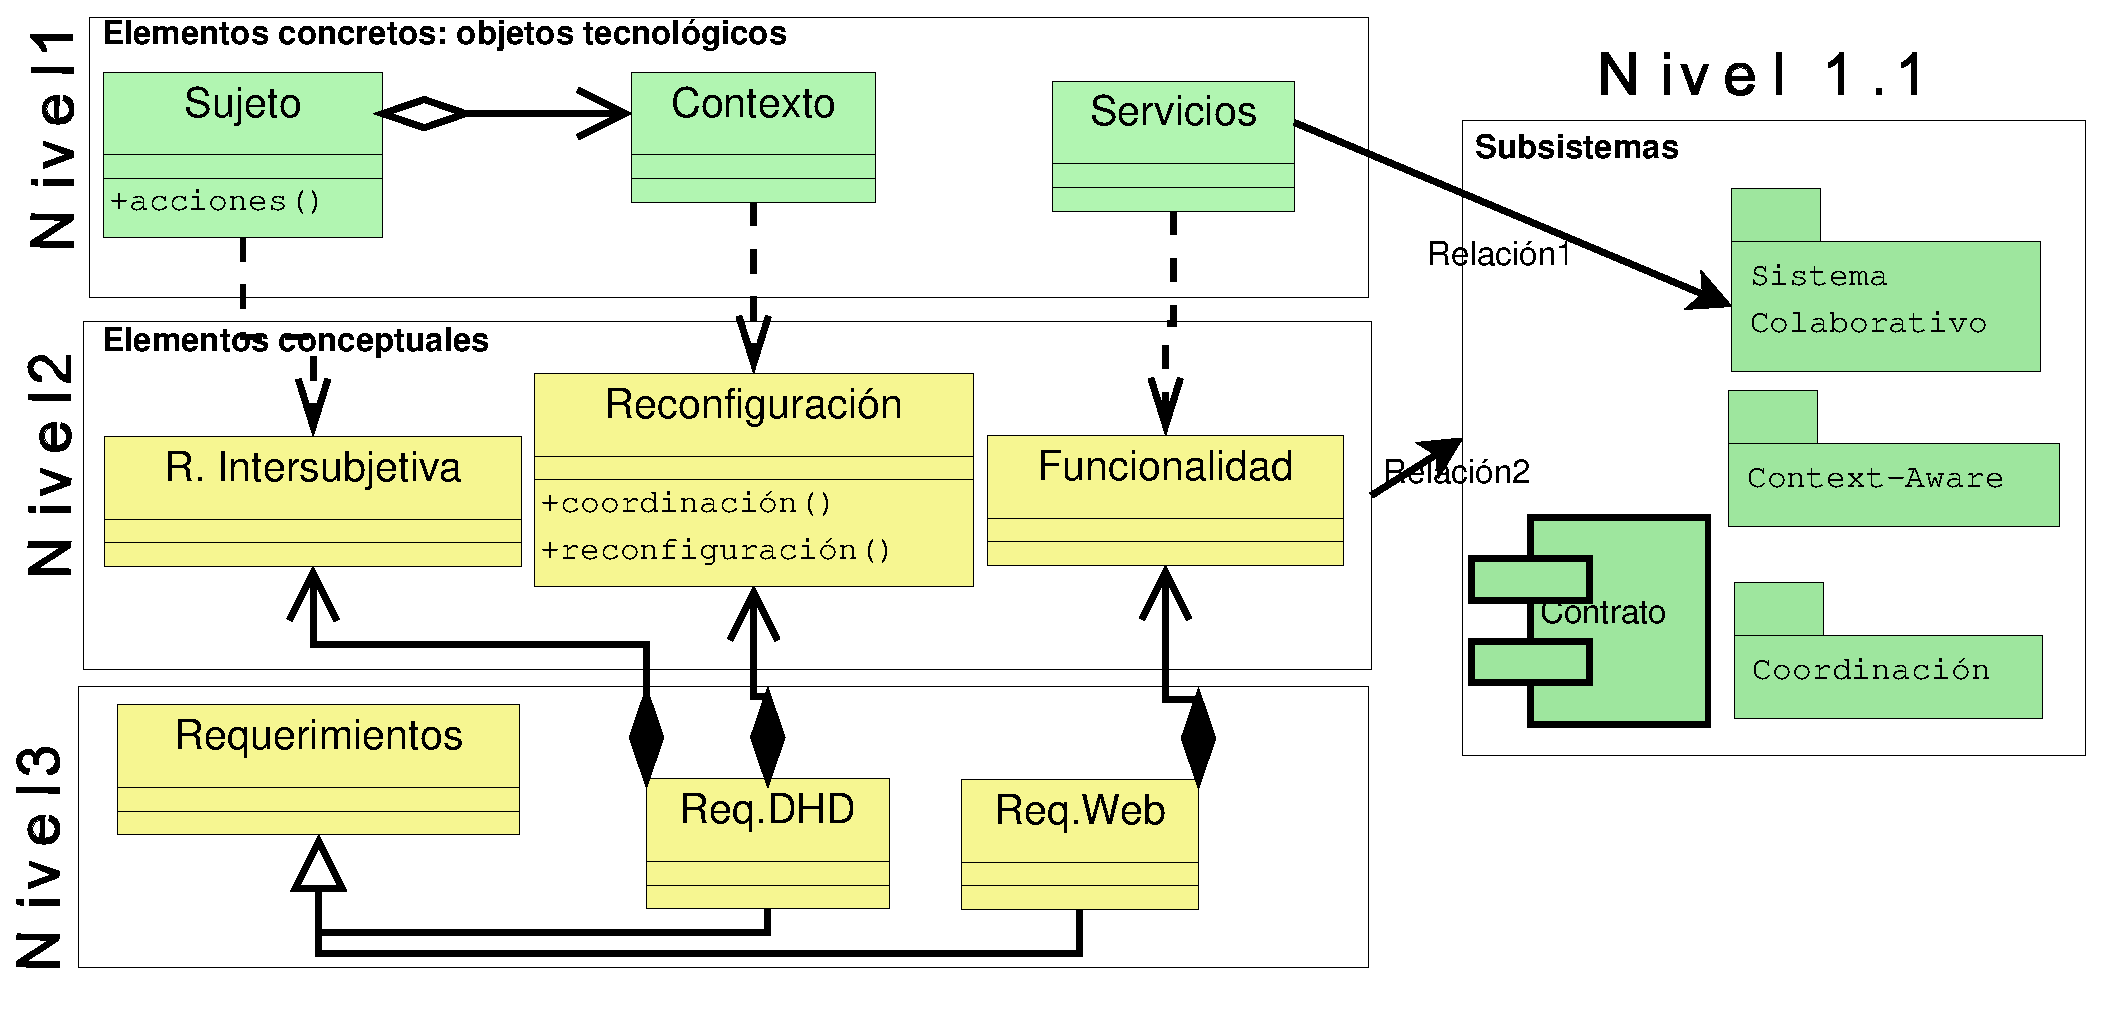
\includegraphics[width=5 in,totalheight=2.3 in] {DHD/RequerimientosDHD}
 % .: 0x0 pixel, 0dpi, 0.00x0.00 cm, bb=
   \caption{Niveles de abstracción y elementos de refinamiento sobre
los RequerimientosDHD} \label{fig: RequerimientosDHD}
\end{center}
\end{figure}


En el nivel 1 se encuentran las componentes tecnológicas que tienen una
influencia directa en la conformación de las componentes del nivel 2. En este
caso se representa con una flecha discontinua la Interactividad DHD
(\textit{Interactividad DHD}) (\ref{relaciones}) tienen una  dependencia de
concretización tecnológica desde los objetos que caracterizan a los sujetos
(\textit{Sujetos}) del DHD. De la misma manera las reconfiguración
que se producen en los DHD depende de la posibiliad de representación y
acciones sobre el contexto. A su vez, todas las funcionalidades computables son
producto de la manipulación que se puedan lograr a partir de las
implementaciones de los servicios.  

Con el propósito de reforzar la definición de requerimientos para los DHD,
el nivel 3 se utiliza para distinguir cuales son los elementos concretos (del
nivel 2) en los cuales se basan los límites impuestos al concepto del Dispositivo Hipermedial
Dinámico para hacer posible las representaciones computacionales. 

Por otro lado, en el nivel 1.1 se encuentran los elementos que se agregan a los
del nivel 1 para aportar mejor representación, diseño e implementación de
los RequerimientosDHD. Se plantea que las formas de relacionamiento de estos elementos con los anteriores establecen un modelo que fija el diseño
computacional del DHD justificando los argumentos expuestos en la definición del plano 3
(\ref{plano3}). Estructuralmente, dicho modelo respeta la lógica de que
indefectiblemente debe existir un nuevo nivel de representación de las
funcionalidades, requerimientos y requisitos en la construcción del DHD visto desde el aporte multidisciplinario.

La figura \ref{requerimientosdhd} muestra tres subsistemas relacionados dentro del
nivel 1.1 y una componente (\textit{Contrato}) que tendrá un protagonismo
conceptual importante en esta tesis. Las cuestiones de diseño, implementación
y uso de los subsistemas serán tratadas en los capítulos siguientes. Se desarrollará cómo a partir de un framework colaborativo Web son utilizados sus
servicios bases (relación 1). A su vez, los elementos de reconfiguración
estarán ligados a un mecanismo de coordinación a partir de la intervención de
los contratos y se tendrá otro subsistema encargado de la
manipulación y representación de contexto. Estos mismos elementos
intervendrán en el tratamiento de la Interacividad DHD donde su
nivel de expresión quedará supeditado a la forma de relacionarlos.

\begin{figure}[h]
\begin{center}
 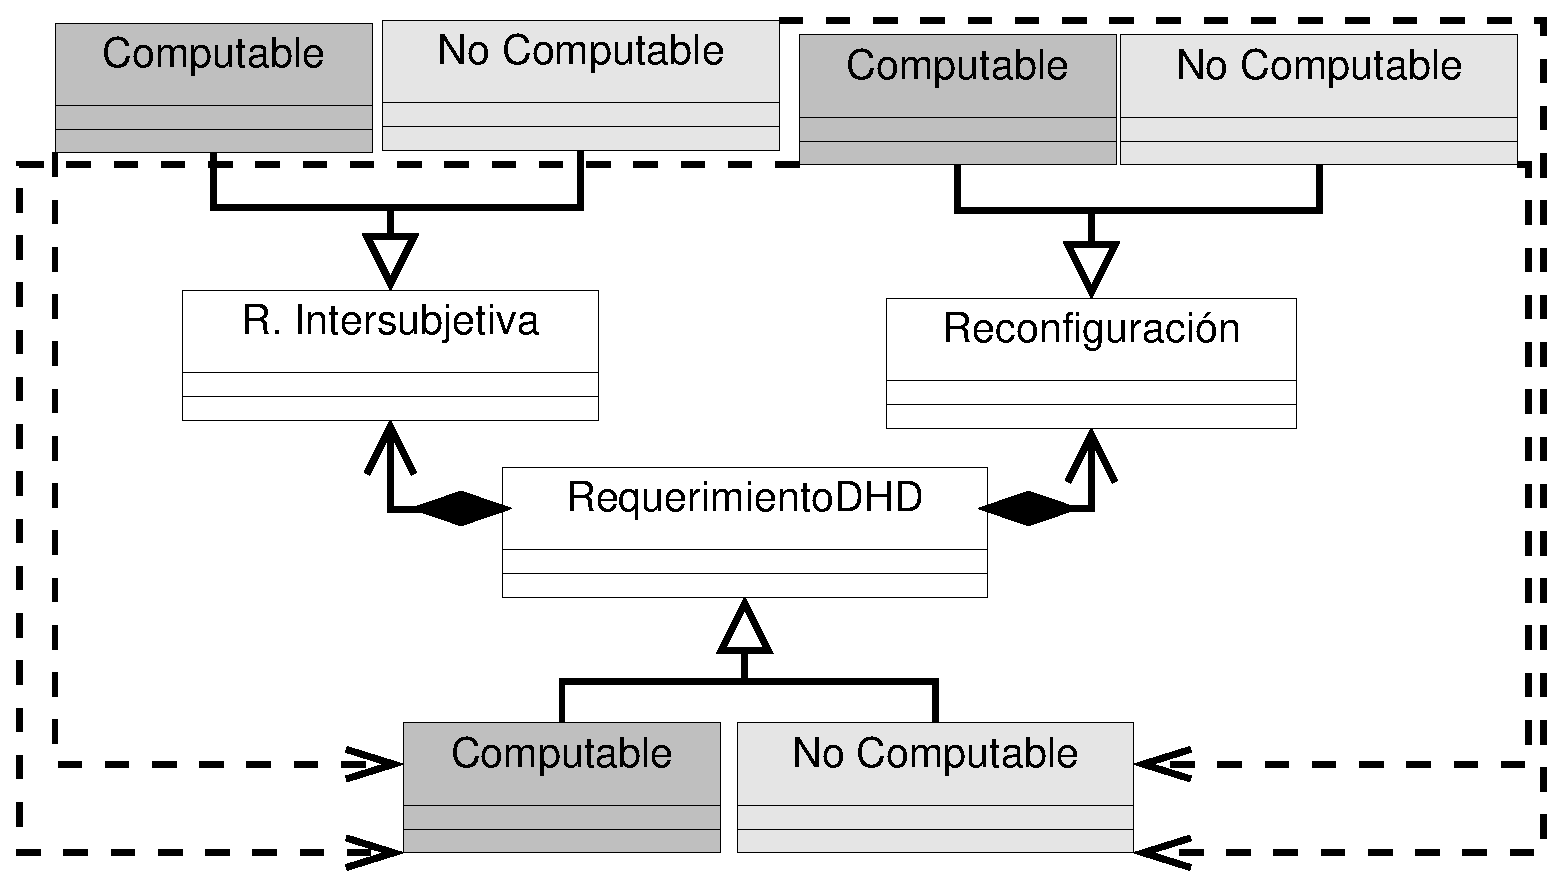
\includegraphics[width=3 in,totalheight=3 in] {DHD/RequerimientosDHD2}
 % .: 0x0 pixel, 0dpi, 0.00x0.00 cm, bb=
\caption{Estructura del RequerimientoDHD} \label{RequerimientosDHD2}
\end{center}
 \end{figure}

Finalmente hemos arribado a una representación sobre la
estructura que determina a los Requerimientos del DHD donde se expresa la necesidad de considerar permanentemente lo no computable para dar sentido a lo computable y efectuar las distinciones de Requerimientos tecnológicos correspondientes a través de sucesivos refinamientos. 


\colorbox{yellow}{Agregar lo del paper sobre requrimientos para C-AS  paper(135)}


\section{Conclusiones}

En este capítulo se hizo necesario exponer integralmente el marco conceptual del DHD para educar, investigar y/o producir desarrollado bajo una metodología de trabajo interdisciplinar con la finalidad de situar los límites disciplinares de la presente Tesis.
A partir de una observación centrada en lo que puede ser computable o no, fue posible aplicar la Teoría de Requerimientos para avanzar metodológicamente en el abordaje del tratamiento tecnológico. Entonces, se logró identificar un patrón que expresa la
estructura de los RequerimientosDHD. Este avance posibilita y postula con claridad el recorte disciplinar necesario al concepto general del DHD, para comprender el desarrollo de los siguientes capítulos que configuran este escrito. 
